% Created by tikzDevice version 0.12.6 on 2025-12-06 13:26:14
% !TEX encoding = UTF-8 Unicode
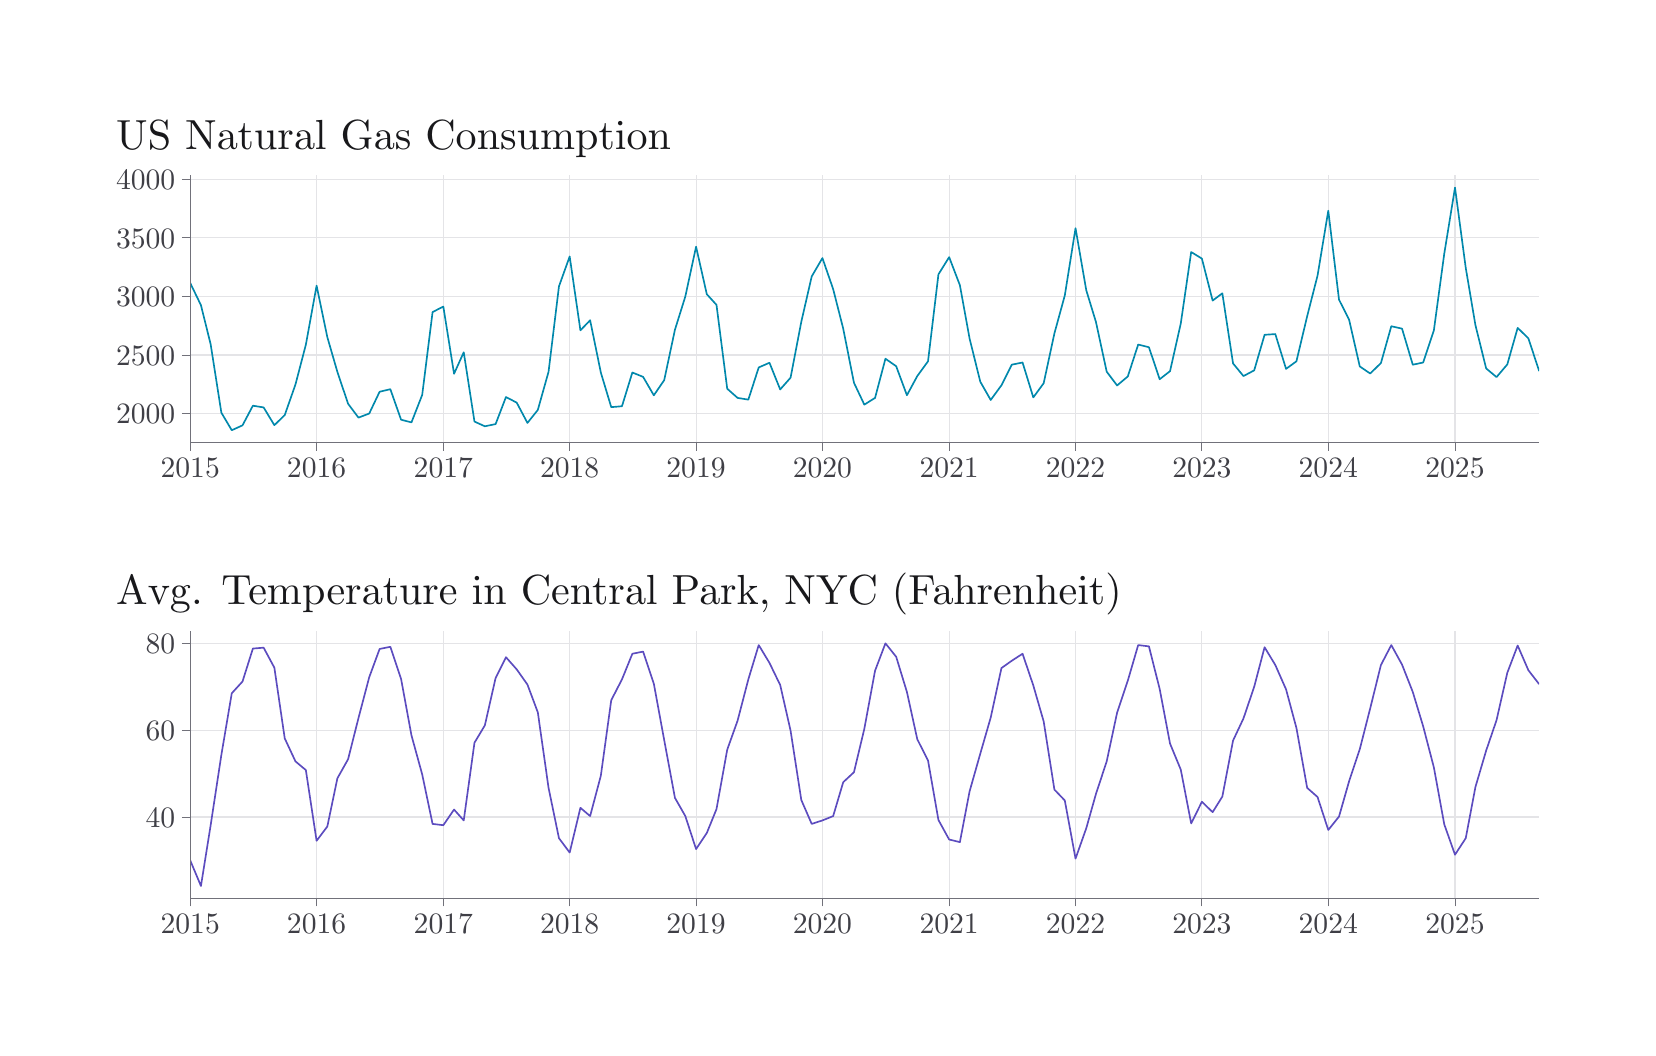
\begin{tikzpicture}[x=1pt,y=1pt]
\definecolor{fillColor}{RGB}{255,255,255}
\path[use as bounding box,fill=fillColor] (0,0) rectangle (578.16,361.35);
\begin{scope}
\path[clip] (  0.00,  0.00) rectangle (578.16,361.35);
\definecolor{drawColor}{RGB}{255,255,255}

\path[draw=drawColor,line width= 0.7pt,line join=round,line cap=round,fill=fillColor] (  0.00, -0.00) rectangle (578.16,361.35);
\end{scope}
\begin{scope}
\path[clip] ( 16.00,180.67) rectangle (562.16,345.35);
\definecolor{drawColor}{RGB}{255,255,255}
\definecolor{fillColor}{RGB}{255,255,255}

\path[draw=drawColor,line width= 0.6pt,line join=round,line cap=round,fill=fillColor] ( 16.00,180.67) rectangle (562.16,345.35);
\end{scope}
\begin{scope}
\path[clip] ( 16.00, 16.00) rectangle (562.16,180.68);
\definecolor{drawColor}{RGB}{255,255,255}
\definecolor{fillColor}{RGB}{255,255,255}

\path[draw=drawColor,line width= 0.6pt,line join=round,line cap=round,fill=fillColor] ( 16.00, 16.00) rectangle (562.16,180.68);
\end{scope}
\begin{scope}
\path[clip] ( 58.73,211.50) rectangle (546.16,307.94);
\definecolor{drawColor}{RGB}{255,255,255}
\definecolor{fillColor}{RGB}{255,255,255}

\path[draw=drawColor,line width= 0.6pt,line join=round,line cap=round,fill=fillColor] ( 58.73,211.50) rectangle (546.16,307.94);
\definecolor{drawColor}{RGB}{228,228,231}

\path[draw=drawColor,line width= 0.4pt,line join=round] ( 58.73,221.89) --
	(546.16,221.89);

\path[draw=drawColor,line width= 0.4pt,line join=round] ( 58.73,243.06) --
	(546.16,243.06);

\path[draw=drawColor,line width= 0.4pt,line join=round] ( 58.73,264.23) --
	(546.16,264.23);

\path[draw=drawColor,line width= 0.4pt,line join=round] ( 58.73,285.41) --
	(546.16,285.41);

\path[draw=drawColor,line width= 0.4pt,line join=round] ( 58.73,306.58) --
	(546.16,306.58);

\path[draw=drawColor,line width= 0.4pt,line join=round] ( 58.73,211.50) --
	( 58.73,307.94);

\path[draw=drawColor,line width= 0.4pt,line join=round] (104.40,211.50) --
	(104.40,307.94);

\path[draw=drawColor,line width= 0.4pt,line join=round] (150.19,211.50) --
	(150.19,307.94);

\path[draw=drawColor,line width= 0.4pt,line join=round] (195.85,211.50) --
	(195.85,307.94);

\path[draw=drawColor,line width= 0.4pt,line join=round] (241.52,211.50) --
	(241.52,307.94);

\path[draw=drawColor,line width= 0.4pt,line join=round] (287.18,211.50) --
	(287.18,307.94);

\path[draw=drawColor,line width= 0.4pt,line join=round] (332.97,211.50) --
	(332.97,307.94);

\path[draw=drawColor,line width= 0.4pt,line join=round] (378.64,211.50) --
	(378.64,307.94);

\path[draw=drawColor,line width= 0.4pt,line join=round] (424.30,211.50) --
	(424.30,307.94);

\path[draw=drawColor,line width= 0.4pt,line join=round] (469.97,211.50) --
	(469.97,307.94);

\path[draw=drawColor,line width= 0.4pt,line join=round] (515.76,211.50) --
	(515.76,307.94);
\definecolor{drawColor}{RGB}{1,136,172}

\path[draw=drawColor,line width= 0.6pt,line join=round] ( 58.73,269.10) --
	( 62.61,261.07) --
	( 66.12,246.93) --
	( 69.99,222.22) --
	( 73.75,215.88) --
	( 77.63,217.65) --
	( 81.38,224.75) --
	( 85.26,224.12) --
	( 89.14,217.71) --
	( 92.89,221.35) --
	( 96.77,232.43) --
	(100.52,246.79) --
	(104.40,268.12) --
	(108.28,249.51) --
	(111.91,236.97) --
	(115.78,225.43) --
	(119.54,220.44) --
	(123.42,221.92) --
	(127.17,229.79) --
	(131.05,230.71) --
	(134.93,219.68) --
	(138.68,218.72) --
	(142.56,228.64) --
	(146.31,258.57) --
	(150.19,260.58) --
	(154.07,236.29) --
	(157.57,244.05) --
	(161.45,219.01) --
	(165.20,217.31) --
	(169.08,218.09) --
	(172.83,227.88) --
	(176.71,225.86) --
	(180.59,218.52) --
	(184.34,223.22) --
	(188.22,237.02) --
	(191.98,267.87) --
	(195.85,278.67) --
	(199.73,251.98) --
	(203.24,255.62) --
	(207.11,236.73) --
	(210.87,224.22) --
	(214.75,224.56) --
	(218.50,236.74) --
	(222.38,235.17) --
	(226.26,228.50) --
	(230.01,233.99) --
	(233.89,252.20) --
	(237.64,264.21) --
	(241.52,282.20) --
	(245.40,265.04) --
	(248.90,261.18) --
	(252.78,230.88) --
	(256.53,227.56) --
	(260.41,226.94) --
	(264.16,238.57) --
	(268.04,240.26) --
	(271.92,230.62) --
	(275.67,234.87) --
	(279.55,255.08) --
	(283.31,271.46) --
	(287.18,278.09) --
	(291.06,266.87) --
	(294.69,252.61) --
	(298.57,233.05) --
	(302.32,225.13) --
	(306.20,227.57) --
	(309.95,241.72) --
	(313.83,239.01) --
	(317.71,228.53) --
	(321.46,235.46) --
	(325.34,240.80) --
	(329.10,272.20) --
	(332.97,278.43) --
	(336.85,268.29) --
	(340.36,248.99) --
	(344.23,233.39) --
	(347.99,226.82) --
	(351.87,232.13) --
	(355.62,239.57) --
	(359.50,240.36) --
	(363.38,227.74) --
	(367.13,232.87) --
	(371.01,250.89) --
	(374.76,264.58) --
	(378.64,288.88) --
	(382.52,266.45) --
	(386.02,254.99) --
	(389.90,237.05) --
	(393.65,232.06) --
	(397.53,235.31) --
	(401.28,246.85) --
	(405.16,245.88) --
	(409.04,234.31) --
	(412.79,237.23) --
	(416.67,254.45) --
	(420.43,280.28) --
	(424.30,277.90) --
	(428.18,262.73) --
	(431.69,265.35) --
	(435.56,240.02) --
	(439.32,235.45) --
	(443.20,237.52) --
	(446.95,250.36) --
	(450.83,250.63) --
	(454.71,238.05) --
	(458.46,240.79) --
	(462.34,257.08) --
	(466.09,271.76) --
	(469.97,295.21) --
	(473.85,263.05) --
	(477.48,255.88) --
	(481.35,238.94) --
	(485.11,236.37) --
	(488.99,240.15) --
	(492.74,253.46) --
	(496.62,252.59) --
	(500.50,239.56) --
	(504.25,240.35) --
	(508.13,252.01) --
	(511.88,279.69) --
	(515.76,303.55) --
	(519.64,274.56) --
	(523.14,253.86) --
	(527.02,238.21) --
	(530.77,235.08) --
	(534.65,239.66) --
	(538.40,252.86) --
	(542.28,249.09) --
	(546.16,237.27);
\end{scope}
\begin{scope}
\path[clip] (  0.00,  0.00) rectangle (578.16,361.35);
\definecolor{drawColor}{RGB}{113,113,122}

\path[draw=drawColor,line width= 0.3pt,line join=round] ( 58.73,211.50) --
	( 58.73,307.94);
\end{scope}
\begin{scope}
\path[clip] (  0.00,  0.00) rectangle (578.16,361.35);
\definecolor{drawColor}{RGB}{63,63,70}

\node[text=drawColor,anchor=base east,inner sep=0pt, outer sep=0pt, scale=  1.07] at ( 53.33,218.21) {2000};

\node[text=drawColor,anchor=base east,inner sep=0pt, outer sep=0pt, scale=  1.07] at ( 53.33,239.39) {2500};

\node[text=drawColor,anchor=base east,inner sep=0pt, outer sep=0pt, scale=  1.07] at ( 53.33,260.56) {3000};

\node[text=drawColor,anchor=base east,inner sep=0pt, outer sep=0pt, scale=  1.07] at ( 53.33,281.73) {3500};

\node[text=drawColor,anchor=base east,inner sep=0pt, outer sep=0pt, scale=  1.07] at ( 53.33,302.91) {4000};
\end{scope}
\begin{scope}
\path[clip] (  0.00,  0.00) rectangle (578.16,361.35);
\definecolor{drawColor}{RGB}{113,113,122}

\path[draw=drawColor,line width= 0.3pt,line join=round] ( 55.73,221.89) --
	( 58.73,221.89);

\path[draw=drawColor,line width= 0.3pt,line join=round] ( 55.73,243.06) --
	( 58.73,243.06);

\path[draw=drawColor,line width= 0.3pt,line join=round] ( 55.73,264.23) --
	( 58.73,264.23);

\path[draw=drawColor,line width= 0.3pt,line join=round] ( 55.73,285.41) --
	( 58.73,285.41);

\path[draw=drawColor,line width= 0.3pt,line join=round] ( 55.73,306.58) --
	( 58.73,306.58);
\end{scope}
\begin{scope}
\path[clip] (  0.00,  0.00) rectangle (578.16,361.35);
\definecolor{drawColor}{RGB}{113,113,122}

\path[draw=drawColor,line width= 0.3pt,line join=round] ( 58.73,211.50) --
	(546.16,211.50);
\end{scope}
\begin{scope}
\path[clip] (  0.00,  0.00) rectangle (578.16,361.35);
\definecolor{drawColor}{RGB}{113,113,122}

\path[draw=drawColor,line width= 0.3pt,line join=round] ( 58.73,208.50) --
	( 58.73,211.50);

\path[draw=drawColor,line width= 0.3pt,line join=round] (104.40,208.50) --
	(104.40,211.50);

\path[draw=drawColor,line width= 0.3pt,line join=round] (150.19,208.50) --
	(150.19,211.50);

\path[draw=drawColor,line width= 0.3pt,line join=round] (195.85,208.50) --
	(195.85,211.50);

\path[draw=drawColor,line width= 0.3pt,line join=round] (241.52,208.50) --
	(241.52,211.50);

\path[draw=drawColor,line width= 0.3pt,line join=round] (287.18,208.50) --
	(287.18,211.50);

\path[draw=drawColor,line width= 0.3pt,line join=round] (332.97,208.50) --
	(332.97,211.50);

\path[draw=drawColor,line width= 0.3pt,line join=round] (378.64,208.50) --
	(378.64,211.50);

\path[draw=drawColor,line width= 0.3pt,line join=round] (424.30,208.50) --
	(424.30,211.50);

\path[draw=drawColor,line width= 0.3pt,line join=round] (469.97,208.50) --
	(469.97,211.50);

\path[draw=drawColor,line width= 0.3pt,line join=round] (515.76,208.50) --
	(515.76,211.50);
\end{scope}
\begin{scope}
\path[clip] (  0.00,  0.00) rectangle (578.16,361.35);
\definecolor{drawColor}{RGB}{63,63,70}

\node[text=drawColor,anchor=base,inner sep=0pt, outer sep=0pt, scale=  1.07] at ( 58.73,198.75) {2015};

\node[text=drawColor,anchor=base,inner sep=0pt, outer sep=0pt, scale=  1.07] at (104.40,198.75) {2016};

\node[text=drawColor,anchor=base,inner sep=0pt, outer sep=0pt, scale=  1.07] at (150.19,198.75) {2017};

\node[text=drawColor,anchor=base,inner sep=0pt, outer sep=0pt, scale=  1.07] at (195.85,198.75) {2018};

\node[text=drawColor,anchor=base,inner sep=0pt, outer sep=0pt, scale=  1.07] at (241.52,198.75) {2019};

\node[text=drawColor,anchor=base,inner sep=0pt, outer sep=0pt, scale=  1.07] at (287.18,198.75) {2020};

\node[text=drawColor,anchor=base,inner sep=0pt, outer sep=0pt, scale=  1.07] at (332.97,198.75) {2021};

\node[text=drawColor,anchor=base,inner sep=0pt, outer sep=0pt, scale=  1.07] at (378.64,198.75) {2022};

\node[text=drawColor,anchor=base,inner sep=0pt, outer sep=0pt, scale=  1.07] at (424.30,198.75) {2023};

\node[text=drawColor,anchor=base,inner sep=0pt, outer sep=0pt, scale=  1.07] at (469.97,198.75) {2024};

\node[text=drawColor,anchor=base,inner sep=0pt, outer sep=0pt, scale=  1.07] at (515.76,198.75) {2025};
\end{scope}
\begin{scope}
\path[clip] (  0.00,  0.00) rectangle (578.16,361.35);
\definecolor{drawColor}{RGB}{24,24,27}

\node[text=drawColor,anchor=base west,inner sep=0pt, outer sep=0pt, scale=  1.52] at ( 32.00,317.41) {US Natural Gas Consumption};
\end{scope}
\begin{scope}
\path[clip] ( 58.73, 46.82) rectangle (546.16,143.26);
\definecolor{drawColor}{RGB}{255,255,255}
\definecolor{fillColor}{RGB}{255,255,255}

\path[draw=drawColor,line width= 0.6pt,line join=round,line cap=round,fill=fillColor] ( 58.73, 46.82) rectangle (546.16,143.26);
\definecolor{drawColor}{RGB}{228,228,231}

\path[draw=drawColor,line width= 0.4pt,line join=round] ( 58.73, 76.14) --
	(546.16, 76.14);

\path[draw=drawColor,line width= 0.4pt,line join=round] ( 58.73,107.51) --
	(546.16,107.51);

\path[draw=drawColor,line width= 0.4pt,line join=round] ( 58.73,138.88) --
	(546.16,138.88);

\path[draw=drawColor,line width= 0.4pt,line join=round] ( 58.73, 46.82) --
	( 58.73,143.26);

\path[draw=drawColor,line width= 0.4pt,line join=round] (104.40, 46.82) --
	(104.40,143.26);

\path[draw=drawColor,line width= 0.4pt,line join=round] (150.19, 46.82) --
	(150.19,143.26);

\path[draw=drawColor,line width= 0.4pt,line join=round] (195.85, 46.82) --
	(195.85,143.26);

\path[draw=drawColor,line width= 0.4pt,line join=round] (241.52, 46.82) --
	(241.52,143.26);

\path[draw=drawColor,line width= 0.4pt,line join=round] (287.18, 46.82) --
	(287.18,143.26);

\path[draw=drawColor,line width= 0.4pt,line join=round] (332.97, 46.82) --
	(332.97,143.26);

\path[draw=drawColor,line width= 0.4pt,line join=round] (378.64, 46.82) --
	(378.64,143.26);

\path[draw=drawColor,line width= 0.4pt,line join=round] (424.30, 46.82) --
	(424.30,143.26);

\path[draw=drawColor,line width= 0.4pt,line join=round] (469.97, 46.82) --
	(469.97,143.26);

\path[draw=drawColor,line width= 0.4pt,line join=round] (515.76, 46.82) --
	(515.76,143.26);
\definecolor{drawColor}{RGB}{92,76,191}

\path[draw=drawColor,line width= 0.6pt,line join=round] ( 58.73, 60.46) --
	( 62.61, 51.21) --
	( 66.12, 73.16) --
	( 69.99, 98.57) --
	( 73.75,120.84) --
	( 77.63,125.08) --
	( 81.38,136.99) --
	( 85.26,137.31) --
	( 89.14,130.09) --
	( 92.89,104.53) --
	( 96.77, 96.22) --
	(100.52, 93.08) --
	(104.40, 67.52) --
	(108.28, 72.69) --
	(111.91, 90.10) --
	(115.78, 97.00) --
	(119.54,111.90) --
	(123.42,126.64) --
	(127.17,136.84) --
	(131.05,137.62) --
	(134.93,126.02) --
	(138.68,105.63) --
	(142.56, 91.51) --
	(146.31, 73.63) --
	(150.19, 73.16) --
	(154.07, 78.81) --
	(157.57, 74.89) --
	(161.45,102.96) --
	(165.20,109.24) --
	(169.08,126.33) --
	(172.83,133.86) --
	(176.71,129.47) --
	(180.59,123.98) --
	(184.34,113.94) --
	(188.22, 86.65) --
	(191.98, 68.46) --
	(195.85, 63.28) --
	(199.73, 79.44) --
	(203.24, 76.46) --
	(207.11, 91.04) --
	(210.87,118.33) --
	(214.75,125.86) --
	(218.50,135.11) --
	(222.38,135.90) --
	(226.26,124.29) --
	(230.01,103.90) --
	(233.89, 83.04) --
	(237.64, 76.46) --
	(241.52, 64.54) --
	(245.40, 70.34) --
	(248.90, 78.97) --
	(252.78,100.45) --
	(256.53,110.96) --
	(260.41,125.86) --
	(264.16,138.25) --
	(268.04,131.82) --
	(271.92,123.82) --
	(275.67,107.35) --
	(279.55, 82.26) --
	(283.31, 73.63) --
	(287.18, 74.89) --
	(291.06, 76.46) --
	(294.69, 88.69) --
	(298.57, 92.30) --
	(302.32,107.98) --
	(306.20,129.00) --
	(309.95,138.88) --
	(313.83,134.02) --
	(317.71,121.31) --
	(321.46,104.22) --
	(325.34, 96.53) --
	(329.10, 75.05) --
	(332.97, 67.99) --
	(336.85, 67.05) --
	(340.36, 85.40) --
	(344.23, 99.04) --
	(347.99,112.06) --
	(351.87,129.94) --
	(355.62,132.60) --
	(359.50,135.11) --
	(363.38,123.66) --
	(367.13,110.65) --
	(371.01, 86.02) --
	(374.76, 82.10) --
	(378.64, 61.09) --
	(382.52, 72.07) --
	(386.02, 84.46) --
	(389.90, 96.22) --
	(393.65,113.78) --
	(397.53,125.39) --
	(401.28,138.25) --
	(405.16,137.78) --
	(409.04,122.41) --
	(412.79,102.65) --
	(416.67, 93.24) --
	(420.43, 73.79) --
	(424.30, 81.63) --
	(428.18, 77.87) --
	(431.69, 83.51) --
	(435.56,103.75) --
	(439.32,111.74) --
	(443.20,123.19) --
	(446.95,137.47) --
	(450.83,131.04) --
	(454.71,122.25) --
	(458.46,108.29) --
	(462.34, 86.65) --
	(466.09, 83.36) --
	(469.97, 71.44) --
	(473.85, 76.30) --
	(477.48, 89.00) --
	(481.35,100.61) --
	(485.11,115.35) --
	(488.99,131.04) --
	(492.74,138.25) --
	(496.62,131.19) --
	(500.50,121.31) --
	(504.25,108.92) --
	(508.13, 94.02) --
	(511.88, 73.48) --
	(515.76, 62.50) --
	(519.64, 68.46) --
	(523.14, 86.96) --
	(527.02,100.14) --
	(530.77,111.12) --
	(534.65,128.21) --
	(538.40,138.09) --
	(542.28,129.15) --
	(546.16,124.13);
\end{scope}
\begin{scope}
\path[clip] (  0.00,  0.00) rectangle (578.16,361.35);
\definecolor{drawColor}{RGB}{113,113,122}

\path[draw=drawColor,line width= 0.3pt,line join=round] ( 58.73, 46.82) --
	( 58.73,143.26);
\end{scope}
\begin{scope}
\path[clip] (  0.00,  0.00) rectangle (578.16,361.35);
\definecolor{drawColor}{RGB}{63,63,70}

\node[text=drawColor,anchor=base east,inner sep=0pt, outer sep=0pt, scale=  1.07] at ( 53.33, 72.47) {40};

\node[text=drawColor,anchor=base east,inner sep=0pt, outer sep=0pt, scale=  1.07] at ( 53.33,103.84) {60};

\node[text=drawColor,anchor=base east,inner sep=0pt, outer sep=0pt, scale=  1.07] at ( 53.33,135.20) {80};
\end{scope}
\begin{scope}
\path[clip] (  0.00,  0.00) rectangle (578.16,361.35);
\definecolor{drawColor}{RGB}{113,113,122}

\path[draw=drawColor,line width= 0.3pt,line join=round] ( 55.73, 76.14) --
	( 58.73, 76.14);

\path[draw=drawColor,line width= 0.3pt,line join=round] ( 55.73,107.51) --
	( 58.73,107.51);

\path[draw=drawColor,line width= 0.3pt,line join=round] ( 55.73,138.88) --
	( 58.73,138.88);
\end{scope}
\begin{scope}
\path[clip] (  0.00,  0.00) rectangle (578.16,361.35);
\definecolor{drawColor}{RGB}{113,113,122}

\path[draw=drawColor,line width= 0.3pt,line join=round] ( 58.73, 46.82) --
	(546.16, 46.82);
\end{scope}
\begin{scope}
\path[clip] (  0.00,  0.00) rectangle (578.16,361.35);
\definecolor{drawColor}{RGB}{113,113,122}

\path[draw=drawColor,line width= 0.3pt,line join=round] ( 58.73, 43.82) --
	( 58.73, 46.82);

\path[draw=drawColor,line width= 0.3pt,line join=round] (104.40, 43.82) --
	(104.40, 46.82);

\path[draw=drawColor,line width= 0.3pt,line join=round] (150.19, 43.82) --
	(150.19, 46.82);

\path[draw=drawColor,line width= 0.3pt,line join=round] (195.85, 43.82) --
	(195.85, 46.82);

\path[draw=drawColor,line width= 0.3pt,line join=round] (241.52, 43.82) --
	(241.52, 46.82);

\path[draw=drawColor,line width= 0.3pt,line join=round] (287.18, 43.82) --
	(287.18, 46.82);

\path[draw=drawColor,line width= 0.3pt,line join=round] (332.97, 43.82) --
	(332.97, 46.82);

\path[draw=drawColor,line width= 0.3pt,line join=round] (378.64, 43.82) --
	(378.64, 46.82);

\path[draw=drawColor,line width= 0.3pt,line join=round] (424.30, 43.82) --
	(424.30, 46.82);

\path[draw=drawColor,line width= 0.3pt,line join=round] (469.97, 43.82) --
	(469.97, 46.82);

\path[draw=drawColor,line width= 0.3pt,line join=round] (515.76, 43.82) --
	(515.76, 46.82);
\end{scope}
\begin{scope}
\path[clip] (  0.00,  0.00) rectangle (578.16,361.35);
\definecolor{drawColor}{RGB}{63,63,70}

\node[text=drawColor,anchor=base,inner sep=0pt, outer sep=0pt, scale=  1.07] at ( 58.73, 34.07) {2015};

\node[text=drawColor,anchor=base,inner sep=0pt, outer sep=0pt, scale=  1.07] at (104.40, 34.07) {2016};

\node[text=drawColor,anchor=base,inner sep=0pt, outer sep=0pt, scale=  1.07] at (150.19, 34.07) {2017};

\node[text=drawColor,anchor=base,inner sep=0pt, outer sep=0pt, scale=  1.07] at (195.85, 34.07) {2018};

\node[text=drawColor,anchor=base,inner sep=0pt, outer sep=0pt, scale=  1.07] at (241.52, 34.07) {2019};

\node[text=drawColor,anchor=base,inner sep=0pt, outer sep=0pt, scale=  1.07] at (287.18, 34.07) {2020};

\node[text=drawColor,anchor=base,inner sep=0pt, outer sep=0pt, scale=  1.07] at (332.97, 34.07) {2021};

\node[text=drawColor,anchor=base,inner sep=0pt, outer sep=0pt, scale=  1.07] at (378.64, 34.07) {2022};

\node[text=drawColor,anchor=base,inner sep=0pt, outer sep=0pt, scale=  1.07] at (424.30, 34.07) {2023};

\node[text=drawColor,anchor=base,inner sep=0pt, outer sep=0pt, scale=  1.07] at (469.97, 34.07) {2024};

\node[text=drawColor,anchor=base,inner sep=0pt, outer sep=0pt, scale=  1.07] at (515.76, 34.07) {2025};
\end{scope}
\begin{scope}
\path[clip] (  0.00,  0.00) rectangle (578.16,361.35);
\definecolor{drawColor}{RGB}{24,24,27}

\node[text=drawColor,anchor=base west,inner sep=0pt, outer sep=0pt, scale=  1.52] at ( 32.00,152.74) {Avg. Temperature in Central Park, NYC (Fahrenheit)};
\end{scope}
\end{tikzpicture}
